%%=============================================================================
%%  ML4D -- First Workshop on Machine Learning for Defense
%%  Author template. Replace the \lipsum[1] filler with your own text.
%%
%%  Class options:
%%    [review]   double-blind: authors hidden, line numbers, page numbers
%%    [final]    camera-ready
%%    [preprint] named authors + banner, for arXiv/internal circulation
%%    [a4paper]  A4 instead of US Letter
%%
%%  Build:  latexmk -pdf main.tex      (or: pdflatex, bibtex, pdflatex x2)
%%
%%  See example-annotated.tex for the same skeleton with guidance notes
%%  instead of filler text.
%%=============================================================================
\documentclass[review]{ml4d}

\usepackage{lipsum}   % PLACEHOLDER TEXT ONLY -- delete once you write the paper

%% --- Optional packages you may want -----------------------------------------
% \usepackage{algorithm}
% \usepackage{algpseudocode}
% \usepackage{siunitx}
% \usepackage{subcaption}

%% --- Handy macros (delete what you do not use) ------------------------------
\newcommand{\vect}[1]{\mathbf{#1}}
\newcommand{\set}[1]{\mathcal{#1}}
\newcommand{\expect}{\mathbb{E}}
\newcommand{\todo}[1]{\textcolor{red}{[TODO: #1]}}

%% --- Front matter -----------------------------------------------------------
\title{Title of Your Paper Goes Here\\ Use a Line Break for Long Titles}

\author{%
  \authorblock{First A. Author}{%
    Institute for Applied Machine Learning\\
    University of Somewhere, Hamburg, Germany\\
    \email{first.author@example.org}}
  \authorsep
  \authorblock{Second B. Author}{%
    Defence Science Laboratory\\
    Somewhere, Country\\
    \email{second.author@example.org}}
  \authorsep
  \authorblock{Third C. Author}{%
    Institute for Applied Machine Learning\\
    University of Somewhere, Hamburg, Germany\\
    \email{third.author@example.org}}
}

%% Optional: appears as an unnumbered footnote on page 1. Delete if not needed.
\distributionstatement{%
  Approved for public release; distribution is unlimited. The views expressed
  are those of the authors and do not necessarily reflect the official policy
  or position of any affiliated organisation.}

%% Optional: overrides the banner text shown in review/preprint mode.
\conference{First Workshop on Machine Learning for Defense (ML4D 2027)}

\begin{document}
\maketitle

\begin{abstract}
\lipsum[1]
\end{abstract}

\keywords{lorem, ipsum, dolor, sit amet, consectetur}

%%-----------------------------------------------------------------------------
\section{Introduction}
%%-----------------------------------------------------------------------------
\lipsum[1]

Cite prior work with the usual commands: a single reference
\cite{lecun2015deep}, a pair \cite{he2016deep,vaswani2017attention}, or a list
\cite{lecun2015deep,szegedy2014intriguing,goodfellow2015explaining}.

\begin{itemize}
  \item Lorem ipsum dolor sit amet, consectetur adipiscing elit;
  \item ut purus elit, vestibulum ut, placerat ac, adipiscing vitae, felis; and
  \item curabitur dictum gravida mauris, nam arcu libero.
\end{itemize}

%% Floats are declared early so they land at the top of a page. Move them next
%% to the text that discusses them once your paper has its final length.
\begin{figure}[t]
  \centering
  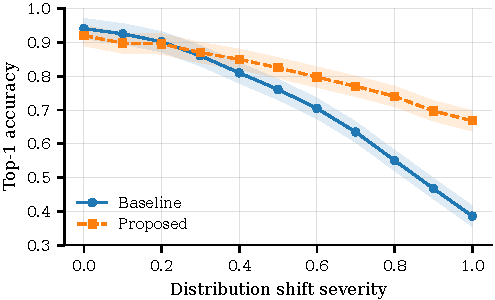
\includegraphics[width=\columnwidth]{figures/example-plot.pdf}
  \caption{Lorem ipsum dolor sit amet, consectetur adipiscing elit.}
  \label{fig:example}
\end{figure}

\begin{figure*}[t]
  \centering
  \fbox{\parbox[c][3.2cm][c]{0.92\textwidth}{\centering
    \textit{Placeholder for a full-width figure. Replace this box with
    \texttt{\textbackslash includegraphics[width=\textbackslash textwidth]\{...\}}.}}}
  \caption{Lorem ipsum dolor sit amet. A double-column figure, produced with
  the \texttt{figure*} environment.}
  \label{fig:wide}
\end{figure*}

%%-----------------------------------------------------------------------------
\section{Related Work}
%%-----------------------------------------------------------------------------
\lipsum[1]

\subsection{A Subsection Heading}
\lipsum[1]

\subsubsection{A Sub-subsection Heading}
\lipsum[1]

\paragraph{A run-in paragraph heading}
\lipsum[1]

%%-----------------------------------------------------------------------------
\section{Method}
%%-----------------------------------------------------------------------------
\lipsum[1]

Display equations are numbered on the right:
%
\begin{equation}
  \label{eq:risk}
  \mathcal{R}_{\mathrm{t}}(f)
    = \expect_{(\vect{x},y)\sim P_{\mathrm{t}}}
      \big[\,\ell\big(f(\vect{x}),\, y\big)\,\big],
\end{equation}
%
and a multi-line derivation is set with \texttt{align}:
%
\begin{align}
  \label{eq:bound}
  \mathcal{R}_{\mathrm{t}}(f)
    &\le \mathcal{R}_{\mathrm{s}}(f)
       + d_{\mathcal{H}}\big(P_{\mathrm{s}}, P_{\mathrm{t}}\big) + \lambda \\
    &\le \widehat{\mathcal{R}}_{\mathrm{s}}(f)
       + \varepsilon(n,\delta)
       + d_{\mathcal{H}}\big(P_{\mathrm{s}}, P_{\mathrm{t}}\big) + \lambda .
\end{align}
%
Refer to equations as \eqref{eq:risk} and \eqref{eq:bound}, to figures as
Fig.~\ref{fig:example} and Fig.~\ref{fig:wide}, and to tables as
Table~\ref{tab:results}.

\begin{theorem}[Informal]
\label{thm:example}
Lorem ipsum dolor sit amet, consectetur adipiscing elit, for any
$\delta \in (0,1)$ and all $f \in \mathcal{F}$.
\end{theorem}

\begin{proof}
Lorem ipsum dolor sit amet.
\end{proof}

\begin{table}[t]
  \centering
  \caption{Lorem ipsum dolor sit amet}
  \label{tab:results}
  \footnotesize
  \begin{tabular}{@{}lccc@{}}
    \toprule
    Method & Accuracy (\%) & Shifted (\%) & Latency (ms) \\
    \midrule
    Lorem            & 94.1 & 61.2 & \phantom{0}8.4 \\
    Ipsum dolor      & 93.8 & 70.5 & \phantom{0}8.4 \\
    Sit amet         & \textbf{94.3} & \textbf{79.1} & 11.2 \\
    \bottomrule
  \end{tabular}
\end{table}

%%-----------------------------------------------------------------------------
\section{Experiments}
%%-----------------------------------------------------------------------------
\lipsum[1]

%%-----------------------------------------------------------------------------
\section{Discussion and Limitations}
%%-----------------------------------------------------------------------------
\lipsum[1]

%%-----------------------------------------------------------------------------
\section{Dual-Use and Ethical Considerations}
%%-----------------------------------------------------------------------------
\lipsum[1]

%%-----------------------------------------------------------------------------
\section{Conclusion}
%%-----------------------------------------------------------------------------
\lipsum[1]

%%-----------------------------------------------------------------------------
\section*{Acknowledgements}
%%-----------------------------------------------------------------------------
Omit this section in the anonymous review version; the \texttt{review} class
option does not remove it for you.

%%-----------------------------------------------------------------------------
%% \balance equalises the two columns on the final page. Uncomment it only
%% once the paper is otherwise finished, and check the result: it misbehaves
%% when a float is still unplaced at that point in the document.
% \balance
\IfFileExists{IEEEtran.bst}{\bibliographystyle{IEEEtran}}{\bibliographystyle{unsrt}}
\bibliography{references}

\end{document}
